\chapter{IoT Gateway}\label{chap:iotgateway}

Das IoT Gateway dient dazu einzelne Messpunkte zusammen zufassen und die Daten danach ins Internet zu übertragen. Als Gateway Hardware nutzen wir die bekannte Embedded Platform Beagle Bone Black. Dies ermöglicht uns auch vorhandene Erweiterungen zu nutzen. Das Gateway arbeitet mit zwei verschiedenen Methoden um die einzelnen Messpunkte abfragen zu können. Einerseits dem CAN-Bus, welcher in der Automobiltechnik sehr verbreitet ist und anderseits eine Bluetooth Smart Schnittstelle um die Sming Messknoten ansprechen zu können. Die Übertragung ins Internet wird mithilfe eines UMTS-Routers gemacht.


%Unser Internet of Things Gateway besteht wiederum aus mehreren Teilen. Die einzelnen Sensoren werden entweder über den CAN-Bus oder an ein Sming angeschlossen. Der CAN-Bus wird von uns über ein BeagleBone Cape mitgelesen. Die Daten des Smings können wir ebenfalls auf dem BeagleBone empfangen. Dies erreichen wir mit Hilfe des Bluetooth Smart USB Dongle BLED112 von Bluegiga, welcher am BeagleBone angeschlossen wird.

\begin{figure}[hbtp]
    \center
    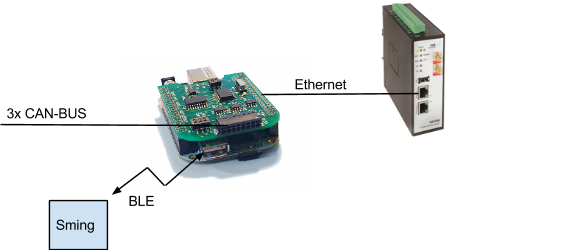
\includegraphics[width=\textwidth]{bilder/aufbau_in_auto.png}
    \caption{Aufbau des IoT Gateways}
    \label{fig:aufbau_iot_gateway}
\end{figure}

\clearpage
\section{Netmodule NetBox NB1600}\label{sec:netbox}
Als UMTS-Router setzen wir auf den Netmodule Router NB1600. Dieser kam schon in unserem Schwerpunkt Mobile Computing beim Semesterprojekt "Smoje" zum Einsatz. Für unseren Einsatzzweck als reine Bridge zwischen Ethernet und UMTS-Netz wird er nicht ausgelastet. Der NB1600 könnte nähmlich auch noch GPS empfangen und als Wlan-Hotspot dienen. Daher besteht hier noch eine Optimierungsmöglichkeit durch den Einsatz eines geigneten USB Dongles der direkt vom Beagle Bone aus auf UMTS zugreifen kann. Dieser zu evaluieren hätte aber den Zeitrahmen für das Projekt gesprengt.

\begin{figure}[hbtp]
	\center
	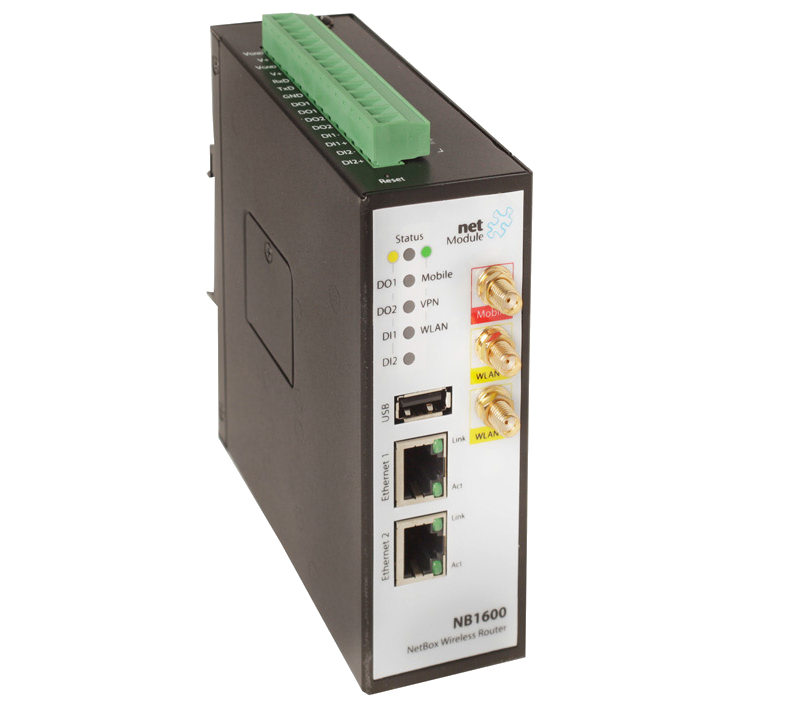
\includegraphics[width=6cm]{bilder/netmodule.png}
	\caption{Foto NetModule NB1600}
	\label{fig:netbox}
\end{figure}


\section{CAN-Cape}
%Als Basis für unsere Software kommt ein BeagleBone Black als Recheneinheit zum Einsatz. Zum Anschliessen der drei CAN-Busse des Fahrzeuges verwenden wir ein von einem Italiener gefertigtes CAN-Cape, dass einfach auf das Beaglebone drauf gesteckt werden kann:

 Der CAN-Bus wird im Bern Formula Student Projekt genutzt um die Steuerbefehle innerhalb des Autos zu übertragen. Es werden drei seperate Verdrathungen geführt. Wir empfangen die Daten der 3 CAN-Busse über das Beagle Bone Black CAN Cape von Tower Tech. Da die ganze Steuerung des Autos über die CAN-Busse läuft haben wir nur lesenden Zugriff. Die Installationsanleitung zum Cape befindet sich im Anhang.

\begin{figure}[hbtp]
	\center
	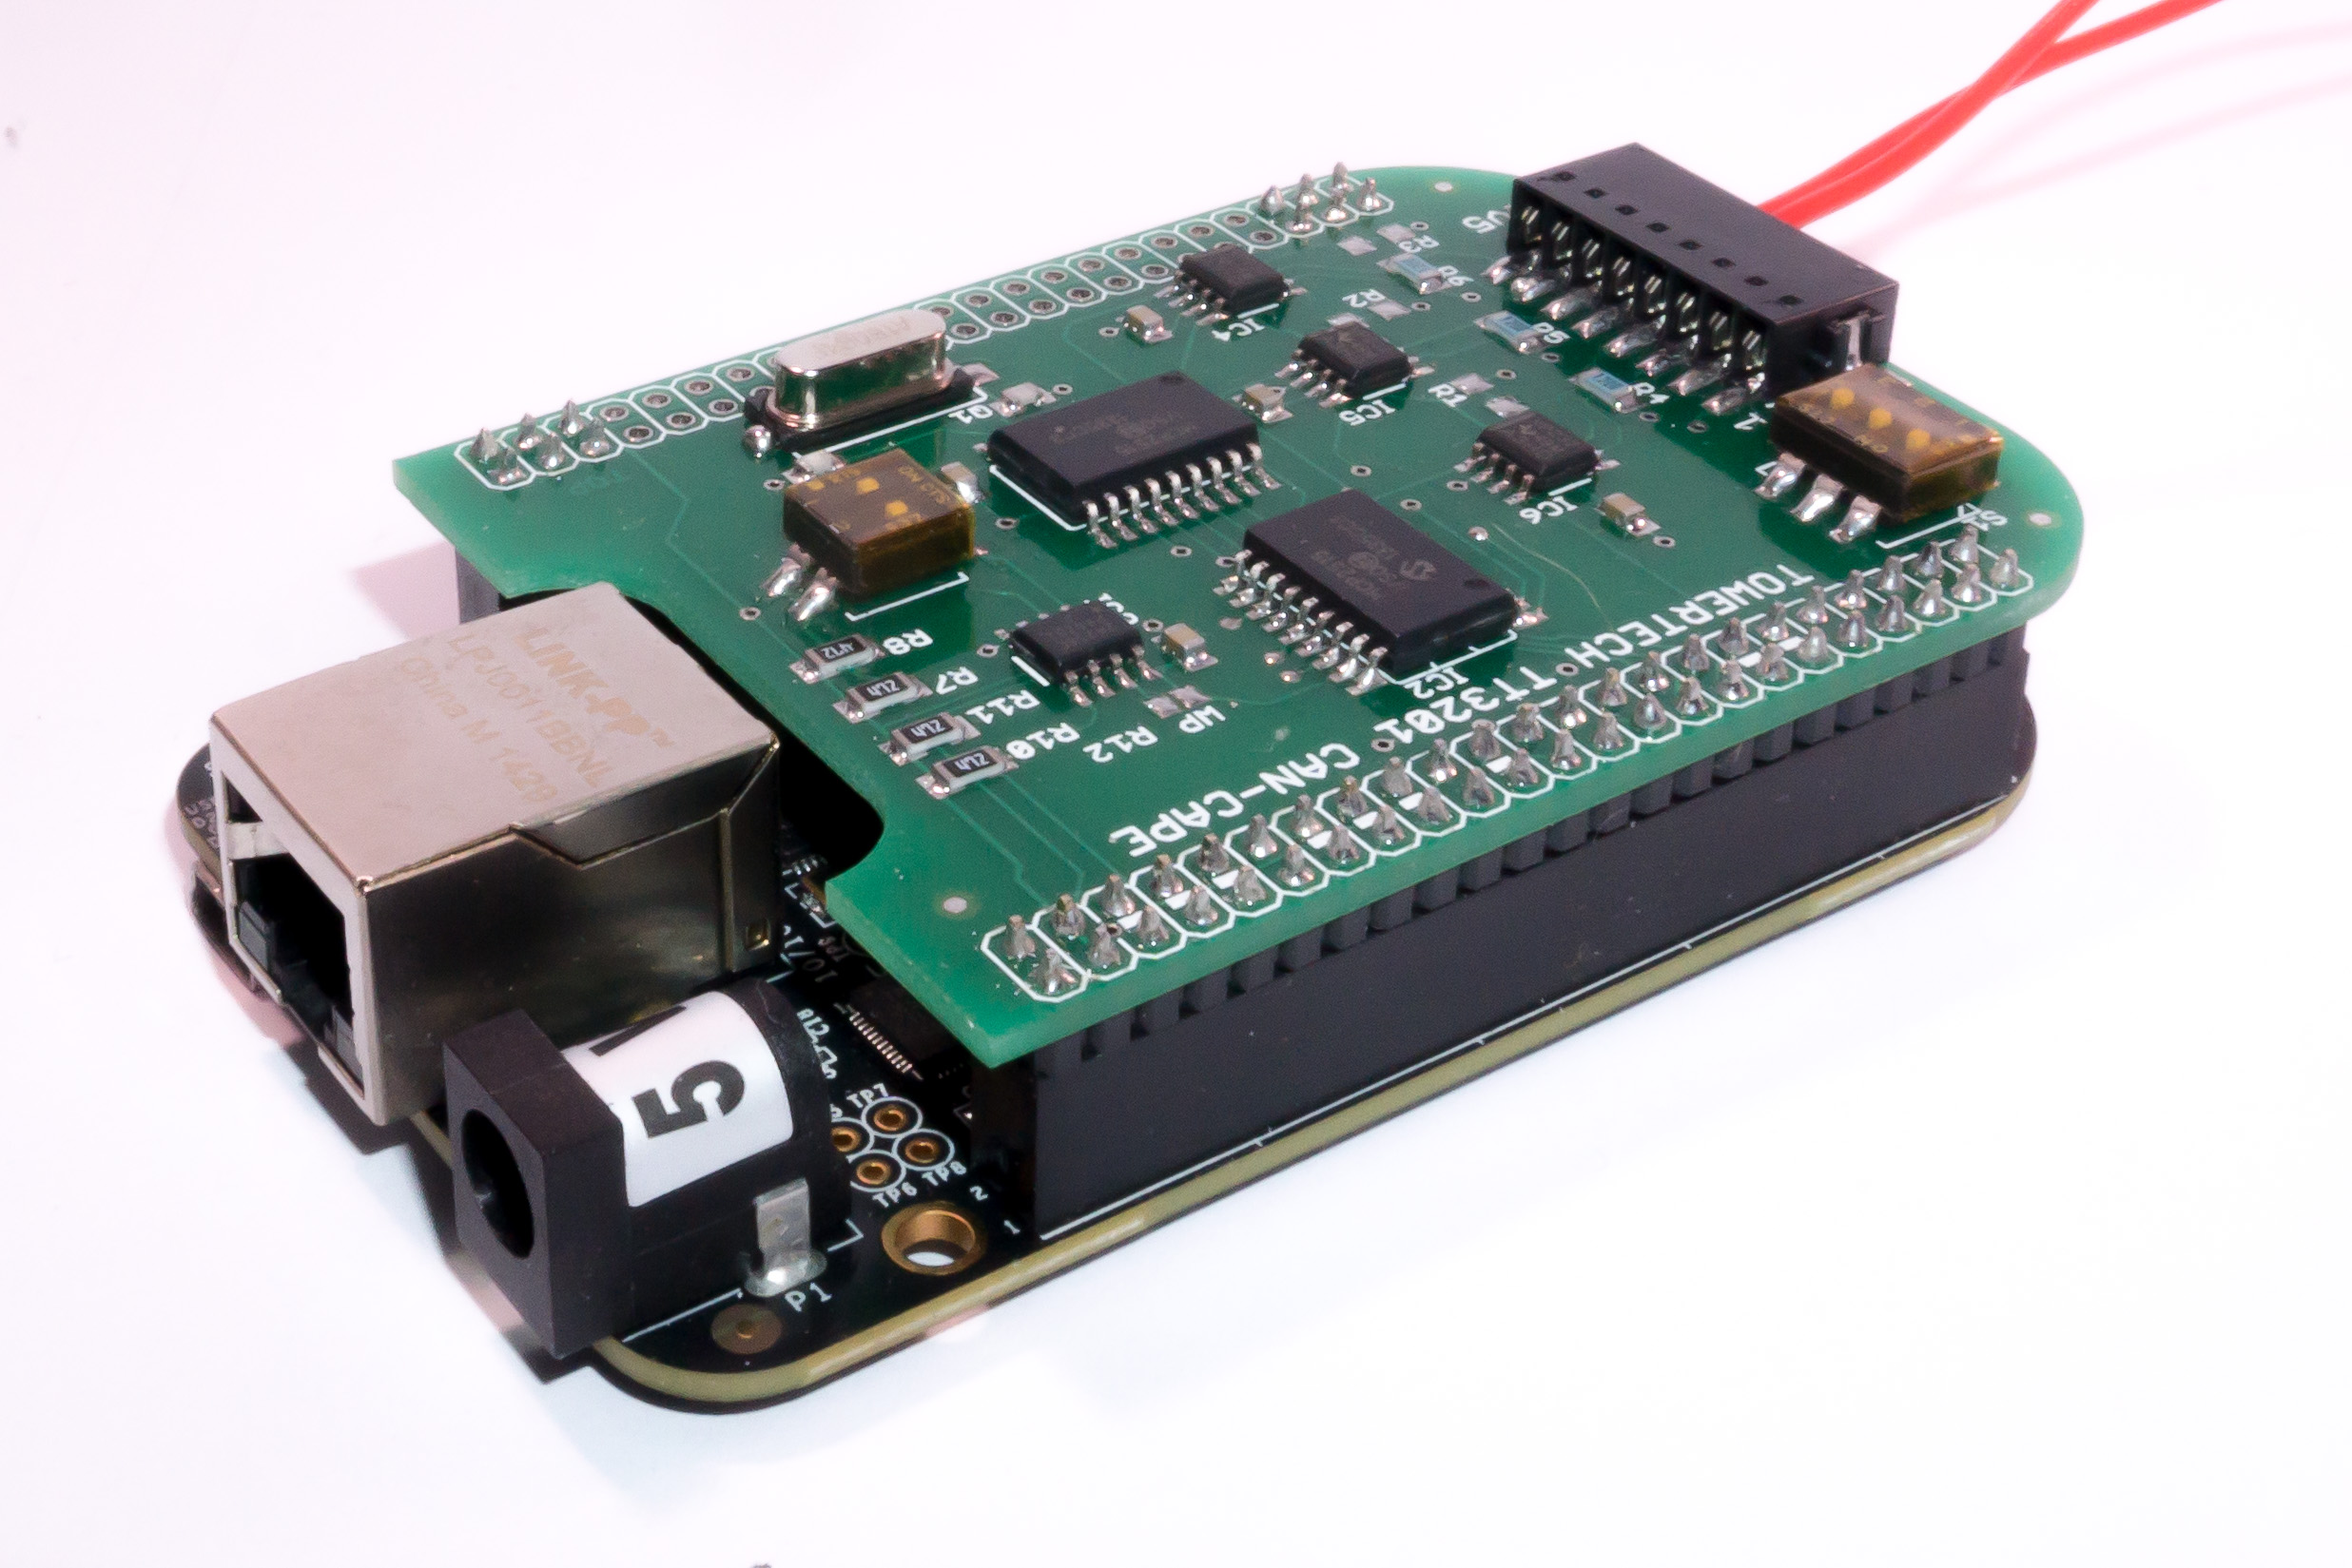
\includegraphics[width=0.8\textwidth]{bilder/foto-4.jpg}
	\caption{Foto CanCape auf Bealge Bone Black}
	\label{fig:CanCape}
\end{figure}

%\textbf{Installationsinstruktionen siehe Anhang.}



\section{BLED112}
Die Schnittstelle zu den Sensoren an den SMINGS ist der USB Dongle BLED112 von Bluegiga. Dieser Mikrocontroller integriert den ganzen Bluetooth Smart Stack, der dank einer API über eine serielle Schnittstelle angesprochen werden kann. Damit ist es nicht nur möglich, die Bluetooth Advertisements der SMINGS zu empfangen, es kann auch mit bis 3\footnote{Die maximale Beschränkung von 3 wurde aus Praxistests mit den Smings festgestellt} Bluetooth 4.0 Geräten verbunden und kommuniziert werden.

Der Bluegiga Chip ist nebst dem auch ein Konkurrenzprodukt zum nRF51 Chip von Nordic, der auf dem Sming zum Einsatz kommt. Wie auch der nRF51 ist der Bluegiga programmierbar, wodurch auch mit diesem autonome smarte Elektronikprojekte realisiert werden können.

Im Anhang findet sich eine Beispiel-Befehlsabfolge, wie sie aktuell zum Verbinden mit dem Smings zum Einsatz kommt. Weitere Informationen wie API Dokumentation, Windows Treiber\footnote{Bei Linux/Mac sind die Treiber bereits im Kernel vorhanden}, etc. finden sich auf folgender Seite:
 \url{https://www.bluegiga.com/en-US/products/bled112-bluetooth-smart-dongle/#documentation}
 
\begin{figure}[hbtp]
	\center
	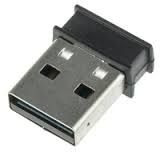
\includegraphics[width=4cm]{bilder/bled112.jpg}
	\caption{Foto BLED112}
	\label{fig:bled112}
\end{figure}

